\documentclass[a4paper]{book}
\usepackage{a4wide}
\usepackage{makeidx}
\usepackage{graphicx}
\usepackage{multicol}
\usepackage{float}
\usepackage{listings}
\usepackage{color}
\usepackage{textcomp}
\usepackage{alltt}
\usepackage{times}
\usepackage{ifpdf}
\ifpdf
\usepackage[pdftex,
            pagebackref=true,
            colorlinks=true,
            linkcolor=blue,
            unicode
           ]{hyperref}
\else
\usepackage[ps2pdf,
            pagebackref=true,
            colorlinks=true,
            linkcolor=blue,
            unicode
           ]{hyperref}
\usepackage{pspicture}
\fi
\usepackage[utf8]{inputenc}
\usepackage{doxygen}
\lstset{language=C++,inputencoding=utf8,basicstyle=\footnotesize,breaklines=true,breakatwhitespace=true,tabsize=8,numbers=left }
\makeindex
\setcounter{tocdepth}{3}
\renewcommand{\footrulewidth}{0.4pt}
\begin{document}
\hypersetup{pageanchor=false}
\begin{titlepage}
\vspace*{7cm}
\begin{center}
{\Large IMFramework \\[1ex]\large 0.1 }\\
\vspace*{1cm}
{\large Generated by Doxygen 1.6.3}\\
\vspace*{0.5cm}
{\small Tue Mar 29 16:28:45 2011}\\
\end{center}
\end{titlepage}
\clearemptydoublepage
\pagenumbering{roman}
\tableofcontents
\clearemptydoublepage
\pagenumbering{arabic}
\hypersetup{pageanchor=true}
\chapter{Class Index}
\section{Class Hierarchy}
This inheritance list is sorted roughly, but not completely, alphabetically:\begin{DoxyCompactList}
\item \contentsline{section}{IMAccount}{\pageref{classIMAccount}}{}
\item \contentsline{section}{IMChannel}{\pageref{classIMChannel}}{}
\item \contentsline{section}{IMClient}{\pageref{classIMClient}}{}
\begin{DoxyCompactList}
\item \contentsline{section}{IRCIMClient}{\pageref{classIRCIMClient}}{}
\item \contentsline{section}{XMPPIMClient}{\pageref{classXMPPIMClient}}{}
\end{DoxyCompactList}
\item \contentsline{section}{IMDaemon}{\pageref{classIMDaemon}}{}
\item \contentsline{section}{IMFramework::IMInterface}{\pageref{classIMFramework_1_1IMInterface}}{}
\begin{DoxyCompactList}
\item \contentsline{section}{IMFramework::Messenger}{\pageref{classIMFramework_1_1Messenger}}{}
\item \contentsline{section}{IMFramework::Presence}{\pageref{classIMFramework_1_1Presence}}{}
\item \contentsline{section}{IMFramework::Query}{\pageref{classIMFramework_1_1Query}}{}
\item \contentsline{section}{IMFramework::Synchronizor}{\pageref{classIMFramework_1_1Synchronizor}}{}
\end{DoxyCompactList}
\item \contentsline{section}{IMService}{\pageref{classIMService}}{}
\item \contentsline{section}{IMServiceTester}{\pageref{classIMServiceTester}}{}
\item \contentsline{section}{irc::IRCChannel}{\pageref{classirc_1_1IRCChannel}}{}
\item \contentsline{section}{irc::IRCClient}{\pageref{classirc_1_1IRCClient}}{}
\item \contentsline{section}{Md5}{\pageref{classMd5}}{}
\item \contentsline{section}{Mime}{\pageref{classMime}}{}
\item \contentsline{section}{Msn}{\pageref{classMsn}}{}
\item \contentsline{section}{MsnAuth}{\pageref{classMsnAuth}}{}
\item \contentsline{section}{MsnChallenge}{\pageref{classMsnChallenge}}{}
\item \contentsline{section}{MsnContact}{\pageref{classMsnContact}}{}
\item \contentsline{section}{MsnContactList}{\pageref{classMsnContactList}}{}
\item \contentsline{section}{MsnSession}{\pageref{classMsnSession}}{}
\item \contentsline{section}{QuerySender}{\pageref{classQuerySender}}{}
\item \contentsline{section}{QueryServer}{\pageref{classQueryServer}}{}
\item \contentsline{section}{SwitchBoardSession}{\pageref{classSwitchBoardSession}}{}
\item \contentsline{section}{SyncTextBox}{\pageref{classSyncTextBox}}{}
\item \contentsline{section}{VRIM}{\pageref{classVRIM}}{}
\end{DoxyCompactList}

\chapter{Class Index}
\section{Class List}
Here are the classes, structs, unions and interfaces with brief descriptions:\begin{DoxyCompactList}
\item\contentsline{section}{\hyperlink{classIMAccount}{IMAccount} }{\pageref{classIMAccount}}{}
\item\contentsline{section}{\hyperlink{classIMChannel}{IMChannel} }{\pageref{classIMChannel}}{}
\item\contentsline{section}{\hyperlink{classIMClient}{IMClient} }{\pageref{classIMClient}}{}
\item\contentsline{section}{\hyperlink{classIMDaemon}{IMDaemon} }{\pageref{classIMDaemon}}{}
\item\contentsline{section}{\hyperlink{classIMFramework_1_1IMInterface}{IMFramework::IMInterface} }{\pageref{classIMFramework_1_1IMInterface}}{}
\item\contentsline{section}{\hyperlink{classIMService}{IMService} }{\pageref{classIMService}}{}
\item\contentsline{section}{\hyperlink{classIMServiceTester}{IMServiceTester} }{\pageref{classIMServiceTester}}{}
\item\contentsline{section}{\hyperlink{classirc_1_1IRCChannel}{irc::IRCChannel} }{\pageref{classirc_1_1IRCChannel}}{}
\item\contentsline{section}{\hyperlink{classirc_1_1IRCClient}{irc::IRCClient} }{\pageref{classirc_1_1IRCClient}}{}
\item\contentsline{section}{\hyperlink{classIRCIMClient}{IRCIMClient} }{\pageref{classIRCIMClient}}{}
\item\contentsline{section}{\hyperlink{classMd5}{Md5} }{\pageref{classMd5}}{}
\item\contentsline{section}{\hyperlink{classIMFramework_1_1Messenger}{IMFramework::Messenger} }{\pageref{classIMFramework_1_1Messenger}}{}
\item\contentsline{section}{\hyperlink{classMime}{Mime} }{\pageref{classMime}}{}
\item\contentsline{section}{\hyperlink{classMsn}{Msn} }{\pageref{classMsn}}{}
\item\contentsline{section}{\hyperlink{classMsnAuth}{MsnAuth} }{\pageref{classMsnAuth}}{}
\item\contentsline{section}{\hyperlink{classMsnChallenge}{MsnChallenge} }{\pageref{classMsnChallenge}}{}
\item\contentsline{section}{\hyperlink{classMsnContact}{MsnContact} }{\pageref{classMsnContact}}{}
\item\contentsline{section}{\hyperlink{classMsnContactList}{MsnContactList} }{\pageref{classMsnContactList}}{}
\item\contentsline{section}{\hyperlink{classMsnSession}{MsnSession} }{\pageref{classMsnSession}}{}
\item\contentsline{section}{\hyperlink{classIMFramework_1_1Presence}{IMFramework::Presence} }{\pageref{classIMFramework_1_1Presence}}{}
\item\contentsline{section}{\hyperlink{classIMFramework_1_1Query}{IMFramework::Query} }{\pageref{classIMFramework_1_1Query}}{}
\item\contentsline{section}{\hyperlink{classQuerySender}{QuerySender} }{\pageref{classQuerySender}}{}
\item\contentsline{section}{\hyperlink{classQueryServer}{QueryServer} }{\pageref{classQueryServer}}{}
\item\contentsline{section}{\hyperlink{classSwitchBoardSession}{SwitchBoardSession} }{\pageref{classSwitchBoardSession}}{}
\item\contentsline{section}{\hyperlink{classIMFramework_1_1Synchronizor}{IMFramework::Synchronizor} }{\pageref{classIMFramework_1_1Synchronizor}}{}
\item\contentsline{section}{\hyperlink{classSyncTextBox}{SyncTextBox} }{\pageref{classSyncTextBox}}{}
\item\contentsline{section}{\hyperlink{classVRIM}{VRIM} }{\pageref{classVRIM}}{}
\item\contentsline{section}{\hyperlink{classXMPPIMClient}{XMPPIMClient} }{\pageref{classXMPPIMClient}}{}
\end{DoxyCompactList}

\chapter{Class Documentation}
\hypertarget{classIMAccount}{
\section{IMAccount Class Reference}
\label{classIMAccount}\index{IMAccount@{IMAccount}}
}
\subsection*{Public Attributes}
\begin{DoxyCompactItemize}
\item 
\hypertarget{classIMAccount_af652309a02d7266cae38f8b9cf75f8af}{
QString {\bfseries accountName}}
\label{classIMAccount_af652309a02d7266cae38f8b9cf75f8af}

\item 
\hypertarget{classIMAccount_a37e95892d4825c7fbd98e173ee42cdba}{
QString {\bfseries type}}
\label{classIMAccount_a37e95892d4825c7fbd98e173ee42cdba}

\item 
\hypertarget{classIMAccount_af0a5bb5484cf39cdb59522bfc2835460}{
QString {\bfseries userName}}
\label{classIMAccount_af0a5bb5484cf39cdb59522bfc2835460}

\item 
\hypertarget{classIMAccount_a78b8b7b36578abb2f477b58fc2698339}{
QString {\bfseries password}}
\label{classIMAccount_a78b8b7b36578abb2f477b58fc2698339}

\item 
\hypertarget{classIMAccount_ab1f168fd1a7ea076426a642e227ab1a8}{
QString {\bfseries server}}
\label{classIMAccount_ab1f168fd1a7ea076426a642e227ab1a8}

\item 
\hypertarget{classIMAccount_a122ffdf1e9c248629abc736939ad6933}{
QString {\bfseries port}}
\label{classIMAccount_a122ffdf1e9c248629abc736939ad6933}

\item 
\hypertarget{classIMAccount_ac4efa2b87d161958f390660082642241}{
QString {\bfseries groups}}
\label{classIMAccount_ac4efa2b87d161958f390660082642241}

\item 
\hypertarget{classIMAccount_a3a0520db9eb280fafc29f9a7035784ca}{
QString {\bfseries memo}}
\label{classIMAccount_a3a0520db9eb280fafc29f9a7035784ca}

\item 
\hypertarget{classIMAccount_a080963b68a91e1885a3f90e8f851efaa}{
QString {\bfseries candos}}
\label{classIMAccount_a080963b68a91e1885a3f90e8f851efaa}

\end{DoxyCompactItemize}


The documentation for this class was generated from the following file:\begin{DoxyCompactItemize}
\item 
adapter/adapter.h\end{DoxyCompactItemize}

\hypertarget{classIMChannel}{
\section{IMChannel Class Reference}
\label{classIMChannel}\index{IMChannel@{IMChannel}}
}
\subsection*{Public Slots}
\begin{DoxyCompactItemize}
\item 
\hypertarget{classIMChannel_a72b1406ad7f4a201227571aacc7c08a5}{
int {\bfseries sendCommand} (QString command)}
\label{classIMChannel_a72b1406ad7f4a201227571aacc7c08a5}

\item 
\hypertarget{classIMChannel_a80baef2b867056f3c5cf8bb77a48fbde}{
int {\bfseries sendCommand} (QString receiver, QString command)}
\label{classIMChannel_a80baef2b867056f3c5cf8bb77a48fbde}

\end{DoxyCompactItemize}
\subsection*{Signals}
\begin{DoxyCompactItemize}
\item 
\hypertarget{classIMChannel_a531782fdd5f721431795ec28d1a28342}{
void {\bfseries statusChanged} (QString participant, QString status)}
\label{classIMChannel_a531782fdd5f721431795ec28d1a28342}

\item 
\hypertarget{classIMChannel_a36b88977bbe65fea6e92269fb5c88742}{
void {\bfseries error} (QString errorType, QString errorMessage)}
\label{classIMChannel_a36b88977bbe65fea6e92269fb5c88742}

\item 
\hypertarget{classIMChannel_a46a6616042149cda70ca6dc5f021e0d5}{
void {\bfseries ready} (bool approved)}
\label{classIMChannel_a46a6616042149cda70ca6dc5f021e0d5}

\end{DoxyCompactItemize}
\subsection*{Public Member Functions}
\begin{DoxyCompactItemize}
\item 
\hypertarget{classIMChannel_afe6d4a5f88d55d1fbccb2dcaf33476a5}{
void {\bfseries initChannel} (QString commandFormat=defaultCommandFormat)}
\label{classIMChannel_afe6d4a5f88d55d1fbccb2dcaf33476a5}

\end{DoxyCompactItemize}


The documentation for this class was generated from the following files:\begin{DoxyCompactItemize}
\item 
protocols/msn/imchannel.h\item 
protocols/msn/imchannel.cpp\end{DoxyCompactItemize}

\hypertarget{classIMClient}{
\section{IMClient Class Reference}
\label{classIMClient}\index{IMClient@{IMClient}}
}
Inheritance diagram for IMClient:\begin{figure}[H]
\begin{center}
\leavevmode
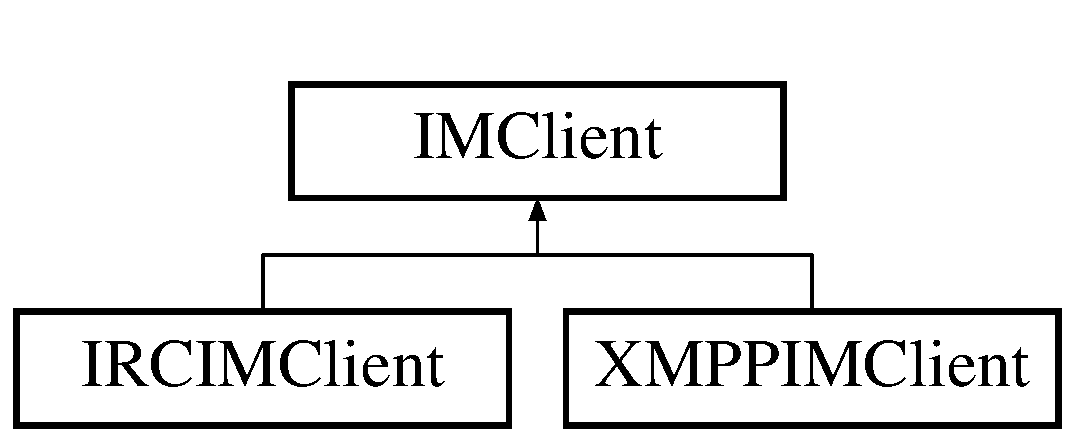
\includegraphics[height=2cm]{classIMClient}
\end{center}
\end{figure}
\subsection*{Public Slots}
\begin{DoxyCompactItemize}
\item 
\hypertarget{classIMClient_a5cb299419096c59ccef91f9dd0ba6331}{
void {\bfseries update} ()}
\label{classIMClient_a5cb299419096c59ccef91f9dd0ba6331}

\end{DoxyCompactItemize}
\subsection*{Signals}
\begin{DoxyCompactItemize}
\item 
\hypertarget{classIMClient_ace3cf2c98aabf8ddb3e520999fec4d33}{
void {\bfseries connected} ()}
\label{classIMClient_ace3cf2c98aabf8ddb3e520999fec4d33}

\item 
\hypertarget{classIMClient_accf2c37275ce59315beed0d2686034c2}{
void {\bfseries disconnected} ()}
\label{classIMClient_accf2c37275ce59315beed0d2686034c2}

\item 
\hypertarget{classIMClient_a0b67d9ebc4be827aac031e813550c058}{
void {\bfseries gotMsg} (QString from, QString message)}
\label{classIMClient_a0b67d9ebc4be827aac031e813550c058}

\item 
\hypertarget{classIMClient_a897dd85750829af5f0dc7dbfb0e9670d}{
void {\bfseries error} (QString errorMsg)}
\label{classIMClient_a897dd85750829af5f0dc7dbfb0e9670d}

\item 
\hypertarget{classIMClient_abe10b1bd73bbdc72e401bf0b1ff33b31}{
void {\bfseries updated} ()}
\label{classIMClient_abe10b1bd73bbdc72e401bf0b1ff33b31}

\end{DoxyCompactItemize}
\subsection*{Public Member Functions}
\begin{DoxyCompactItemize}
\item 
\hypertarget{classIMClient_aee8f4aeb842ed4abb2d9622d539aa59a}{
{\bfseries IMClient} (\hyperlink{classIMAccount}{IMAccount} \&account)}
\label{classIMClient_aee8f4aeb842ed4abb2d9622d539aa59a}

\item 
\hypertarget{classIMClient_ae28370aa8886d1834f02e8a273b3113d}{
virtual bool {\bfseries canDo} (QString serviceType)}
\label{classIMClient_ae28370aa8886d1834f02e8a273b3113d}

\item 
\hypertarget{classIMClient_a7a8f24f0c4d34b7f1f0aa4b74d9a3ea1}{
virtual void {\bfseries login} ()=0}
\label{classIMClient_a7a8f24f0c4d34b7f1f0aa4b74d9a3ea1}

\item 
\hypertarget{classIMClient_a3b10fc13a5712f3eac8693f16e81683d}{
virtual void {\bfseries logout} ()=0}
\label{classIMClient_a3b10fc13a5712f3eac8693f16e81683d}

\item 
\hypertarget{classIMClient_a56f41af0d0b434c9564104aaca012331}{
virtual void {\bfseries sendMsg} (QString target, QString message)=0}
\label{classIMClient_a56f41af0d0b434c9564104aaca012331}

\item 
\hypertarget{classIMClient_a67646bbcbb2c2434f90e5624f05f75d7}{
virtual QStringList {\bfseries getPresence} ()=0}
\label{classIMClient_a67646bbcbb2c2434f90e5624f05f75d7}

\item 
\hypertarget{classIMClient_a1be30f768a0a31e1bafad4915d5f7ac9}{
QString {\bfseries name} ()}
\label{classIMClient_a1be30f768a0a31e1bafad4915d5f7ac9}

\item 
\hypertarget{classIMClient_a73a6b8019fbc05baa39af0bea299cee8}{
virtual bool {\bfseries hasUser} (QString user)}
\label{classIMClient_a73a6b8019fbc05baa39af0bea299cee8}

\end{DoxyCompactItemize}
\subsection*{Public Attributes}
\begin{DoxyCompactItemize}
\item 
\hypertarget{classIMClient_acd536379ac9deeb0b064e2577f10e1da}{
QStringList {\bfseries onlineBuddies}}
\label{classIMClient_acd536379ac9deeb0b064e2577f10e1da}

\item 
\hypertarget{classIMClient_a8bbc41e311653db1693d6a2d784aa4aa}{
bool {\bfseries available}}
\label{classIMClient_a8bbc41e311653db1693d6a2d784aa4aa}

\end{DoxyCompactItemize}
\subsection*{Protected Attributes}
\begin{DoxyCompactItemize}
\item 
\hypertarget{classIMClient_ab37acf43e530eb2b1b08aac0c612d40f}{
QString {\bfseries d\_\-accountName}}
\label{classIMClient_ab37acf43e530eb2b1b08aac0c612d40f}

\item 
\hypertarget{classIMClient_a76ea05c466f863597e7becf7da0704f1}{
QString {\bfseries d\_\-userName}}
\label{classIMClient_a76ea05c466f863597e7becf7da0704f1}

\item 
\hypertarget{classIMClient_ad159062c1294eb3dad03fd64132ca991}{
QString {\bfseries d\_\-password}}
\label{classIMClient_ad159062c1294eb3dad03fd64132ca991}

\item 
\hypertarget{classIMClient_adce305eb1e03f58104960451476a26d7}{
QString {\bfseries d\_\-server}}
\label{classIMClient_adce305eb1e03f58104960451476a26d7}

\item 
\hypertarget{classIMClient_a4f807c21153728b60db53a05b36dd987}{
QString {\bfseries d\_\-port}}
\label{classIMClient_a4f807c21153728b60db53a05b36dd987}

\item 
\hypertarget{classIMClient_af859902b6ff51d784455d7c3a1b360b9}{
QString {\bfseries d\_\-groups}}
\label{classIMClient_af859902b6ff51d784455d7c3a1b360b9}

\item 
\hypertarget{classIMClient_a8fba519da9024ec5bbebee8819fbabb1}{
QString {\bfseries d\_\-memo}}
\label{classIMClient_a8fba519da9024ec5bbebee8819fbabb1}

\item 
\hypertarget{classIMClient_a5b09a04ecba698ecdf1529f7f755ade2}{
QStringList {\bfseries d\_\-canDos}}
\label{classIMClient_a5b09a04ecba698ecdf1529f7f755ade2}

\end{DoxyCompactItemize}


The documentation for this class was generated from the following files:\begin{DoxyCompactItemize}
\item 
adapter/adapter.h\item 
adapter/adapter.cpp\item 
adapter/examples/msg/moc\_\-adapter.cpp\end{DoxyCompactItemize}

\hypertarget{classIMDaemon}{
\section{IMDaemon Class Reference}
\label{classIMDaemon}\index{IMDaemon@{IMDaemon}}
}
\subsection*{Public Slots}
\begin{DoxyCompactItemize}
\item 
\hypertarget{classIMDaemon_a81626921b3a41a0fec35b72855487032}{
void {\bfseries sendMessage} (QString receiver, QString message)}
\label{classIMDaemon_a81626921b3a41a0fec35b72855487032}

\item 
\hypertarget{classIMDaemon_af23e4b8578343cc3610bdfae13c96244}{
void {\bfseries invite} (QString program, QString attachedMessage)}
\label{classIMDaemon_af23e4b8578343cc3610bdfae13c96244}

\end{DoxyCompactItemize}
\subsection*{Signals}
\begin{DoxyCompactItemize}
\item 
\hypertarget{classIMDaemon_af730c723252e6d5713e14ba70f9b2bc6}{
void {\bfseries gotMessage} (QString sender, QString content)}
\label{classIMDaemon_af730c723252e6d5713e14ba70f9b2bc6}

\item 
\hypertarget{classIMDaemon_a2b1a5a17d2e8ad46419af5eb1d31056d}{
void {\bfseries ready} (QString participants)}
\label{classIMDaemon_a2b1a5a17d2e8ad46419af5eb1d31056d}

\end{DoxyCompactItemize}
\subsection*{Public Member Functions}
\begin{DoxyCompactItemize}
\item 
\hypertarget{classIMDaemon_a61999ba31ab441ddd45b6798ae27dbb6}{
{\bfseries IMDaemon} (QWidget $\ast$parent, Qt::WFlags \&flags)}
\label{classIMDaemon_a61999ba31ab441ddd45b6798ae27dbb6}

\end{DoxyCompactItemize}


The documentation for this class was generated from the following files:\begin{DoxyCompactItemize}
\item 
protocols/msn/imdaemon.h\item 
protocols/msn/imdaemon.cpp\end{DoxyCompactItemize}

\hypertarget{classIMFramework_1_1IMInterface}{
\section{IMFramework::IMInterface Class Reference}
\label{classIMFramework_1_1IMInterface}\index{IMFramework::IMInterface@{IMFramework::IMInterface}}
}
Inheritance diagram for IMFramework::IMInterface:\begin{figure}[H]
\begin{center}
\leavevmode
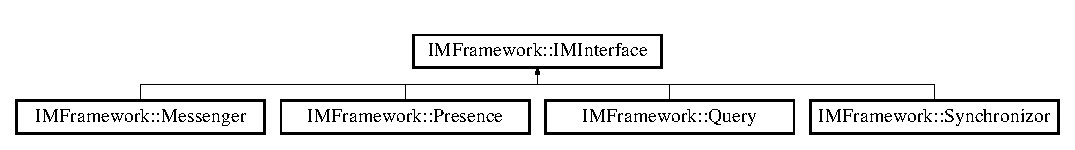
\includegraphics[height=1.56425cm]{classIMFramework_1_1IMInterface}
\end{center}
\end{figure}
\subsection*{Public Member Functions}
\begin{DoxyCompactItemize}
\item 
\hypertarget{classIMFramework_1_1IMInterface_aa4356e86129844a13884416a74caf200}{
{\bfseries IMInterface} (QString type=\char`\"{}\char`\"{})}
\label{classIMFramework_1_1IMInterface_aa4356e86129844a13884416a74caf200}

\item 
\hypertarget{classIMFramework_1_1IMInterface_a0108afbbd4825d97a836e26b4b1b583a}{
void {\bfseries setResourceType} (QString type)}
\label{classIMFramework_1_1IMInterface_a0108afbbd4825d97a836e26b4b1b583a}

\end{DoxyCompactItemize}
\subsection*{Public Attributes}
\begin{DoxyCompactItemize}
\item 
\hypertarget{classIMFramework_1_1IMInterface_aa3c2fb5c152746ec7a24979cec5e7a3f}{
QStringList {\bfseries subscribers}}
\label{classIMFramework_1_1IMInterface_aa3c2fb5c152746ec7a24979cec5e7a3f}

\end{DoxyCompactItemize}
\subsection*{Protected Slots}
\begin{DoxyCompactItemize}
\item 
\hypertarget{classIMFramework_1_1IMInterface_a2c06b029f31cc5fbdd35de2e9b63fecc}{
virtual void {\bfseries gotMsg} (QString from, QString dest, QString msg, long long replyTo)}
\label{classIMFramework_1_1IMInterface_a2c06b029f31cc5fbdd35de2e9b63fecc}

\end{DoxyCompactItemize}
\subsection*{Protected Attributes}
\begin{DoxyCompactItemize}
\item 
\hypertarget{classIMFramework_1_1IMInterface_a03eb5d026d7c48aa42f0a4485287ff5a}{
QString {\bfseries d\_\-resourceType}}
\label{classIMFramework_1_1IMInterface_a03eb5d026d7c48aa42f0a4485287ff5a}

\end{DoxyCompactItemize}
\subsection*{Static Protected Attributes}
\begin{DoxyCompactItemize}
\item 
\hypertarget{classIMFramework_1_1IMInterface_a5ee23f1ea7973b053c3680c7ec37e312}{
static \hyperlink{classIMService}{IMService} $\ast$ {\bfseries d\_\-service} = 0}
\label{classIMFramework_1_1IMInterface_a5ee23f1ea7973b053c3680c7ec37e312}

\end{DoxyCompactItemize}


The documentation for this class was generated from the following files:\begin{DoxyCompactItemize}
\item 
adapter/interface.h\item 
adapter/interface.cpp\end{DoxyCompactItemize}

\hypertarget{classIMService}{
\section{IMService Class Reference}
\label{classIMService}\index{IMService@{IMService}}
}
\subsection*{Signals}
\begin{DoxyCompactItemize}
\item 
\hypertarget{classIMService_a6f1b7156e1d847ecc8820730c26e70c2}{
void {\bfseries gotMsg} (QString from, QString dest, QString message, long long answerTo)}
\label{classIMService_a6f1b7156e1d847ecc8820730c26e70c2}

\item 
\hypertarget{classIMService_a6ea226e19be981791c8e511132ff99fe}{
void {\bfseries updated} ()}
\label{classIMService_a6ea226e19be981791c8e511132ff99fe}

\end{DoxyCompactItemize}
\subsection*{Public Member Functions}
\begin{DoxyCompactItemize}
\item 
\hypertarget{classIMService_ad632df410e1da1384a30123ea6e2cb48}{
void {\bfseries start} ()}
\label{classIMService_ad632df410e1da1384a30123ea6e2cb48}

\item 
\hypertarget{classIMService_ad89df8cc18b93b41a64a0a158d69a997}{
void {\bfseries stop} ()}
\label{classIMService_ad89df8cc18b93b41a64a0a158d69a997}

\item 
\hypertarget{classIMService_a2929379579ad20111ced1c77f8757647}{
long long {\bfseries sendMsg} (QString target, QString app, QString message, \hyperlink{classIMClient}{IMClient} $\ast$client=0)}
\label{classIMService_a2929379579ad20111ced1c77f8757647}

\item 
\hypertarget{classIMService_abe6f85717d7d28d087ec321b65d89c14}{
long long {\bfseries sendMsg} (QStringList targets, QString app, QString message, \hyperlink{classIMClient}{IMClient} $\ast$client=0)}
\label{classIMService_abe6f85717d7d28d087ec321b65d89c14}

\item 
\hypertarget{classIMService_a7a15879d2aeca9cbe4efa7e6f77ed860}{
QString {\bfseries presence} (QString uri)}
\label{classIMService_a7a15879d2aeca9cbe4efa7e6f77ed860}

\item 
\hypertarget{classIMService_a93162cca4207e1bcfbd21ad06d595e5d}{
QStringList {\bfseries friends} (\hyperlink{classIMClient}{IMClient} $\ast$client=0)}
\label{classIMService_a93162cca4207e1bcfbd21ad06d595e5d}

\item 
\hypertarget{classIMService_a9f1c5e4f2bc3e93e308554ec7812a56d}{
QList$<$ \hyperlink{classIMClient}{IMClient} $\ast$ $>$ \& {\bfseries clients} ()}
\label{classIMService_a9f1c5e4f2bc3e93e308554ec7812a56d}

\end{DoxyCompactItemize}


The documentation for this class was generated from the following files:\begin{DoxyCompactItemize}
\item 
adapter/adapter.h\item 
adapter/examples/msg/moc\_\-adapter.cpp\item 
adapter/service.cpp\end{DoxyCompactItemize}

\hypertarget{classIMServiceTester}{
\section{IMServiceTester Class Reference}
\label{classIMServiceTester}\index{IMServiceTester@{IMServiceTester}}
}
\subsection*{Public Slots}
\begin{DoxyCompactItemize}
\item 
\hypertarget{classIMServiceTester_a0e7fd34df3f658ad8fcb551393ac80aa}{
void {\bfseries gotMsg} (QString from, QString message, long answerTo, \hyperlink{classIMClient}{IMClient} $\ast$client)}
\label{classIMServiceTester_a0e7fd34df3f658ad8fcb551393ac80aa}

\end{DoxyCompactItemize}


The documentation for this class was generated from the following file:\begin{DoxyCompactItemize}
\item 
adapter/adapter.h\end{DoxyCompactItemize}

\hypertarget{classirc_1_1IRCChannel}{
\section{irc::IRCChannel Class Reference}
\label{classirc_1_1IRCChannel}\index{irc::IRCChannel@{irc::IRCChannel}}
}
\subsection*{Public Attributes}
\begin{DoxyCompactItemize}
\item 
\hypertarget{classirc_1_1IRCChannel_a4310391332e0e09d792aae41e7110e3a}{
QString {\bfseries d\_\-name}}
\label{classirc_1_1IRCChannel_a4310391332e0e09d792aae41e7110e3a}

\item 
\hypertarget{classirc_1_1IRCChannel_a76cf6dfa688d9029549ca09369bc32a0}{
QString {\bfseries d\_\-description}}
\label{classirc_1_1IRCChannel_a76cf6dfa688d9029549ca09369bc32a0}

\item 
\hypertarget{classirc_1_1IRCChannel_a4b50363dbeb46cc90324114e28cace24}{
int {\bfseries d\_\-headCount}}
\label{classirc_1_1IRCChannel_a4b50363dbeb46cc90324114e28cace24}

\item 
\hypertarget{classirc_1_1IRCChannel_af6d33bb978963b9abfc0fa03eebcc567}{
QStringList {\bfseries d\_\-users}}
\label{classirc_1_1IRCChannel_af6d33bb978963b9abfc0fa03eebcc567}

\end{DoxyCompactItemize}


The documentation for this class was generated from the following file:\begin{DoxyCompactItemize}
\item 
protocols/irc/irc.h\end{DoxyCompactItemize}

\hypertarget{classirc_1_1IRCClient}{
\section{irc::IRCClient Class Reference}
\label{classirc_1_1IRCClient}\index{irc::IRCClient@{irc::IRCClient}}
}
\subsection*{Signals}
\begin{DoxyCompactItemize}
\item 
\hypertarget{classirc_1_1IRCClient_a9e5b75e20a192457f4cdf819b294a8c3}{
void {\bfseries message} (QString from, QString fromURI, QString receiver, QString msg)}
\label{classirc_1_1IRCClient_a9e5b75e20a192457f4cdf819b294a8c3}

\item 
\hypertarget{classirc_1_1IRCClient_afe82b1dfb3e89b99a3113be1a1e03e09}{
void {\bfseries notification} (QString msg)}
\label{classirc_1_1IRCClient_afe82b1dfb3e89b99a3113be1a1e03e09}

\item 
\hypertarget{classirc_1_1IRCClient_a6eb42da585b279e552ed39841b7ae39c}{
void {\bfseries invitation} (QString from, QString toChannel)}
\label{classirc_1_1IRCClient_a6eb42da585b279e552ed39841b7ae39c}

\item 
\hypertarget{classirc_1_1IRCClient_a5ab1f6de72ef1092bbdbfd92e5c5847a}{
void {\bfseries connected} ()}
\label{classirc_1_1IRCClient_a5ab1f6de72ef1092bbdbfd92e5c5847a}

\item 
\hypertarget{classirc_1_1IRCClient_a404b289697f4d575269c43a809a70f2c}{
void {\bfseries ping} (QString \&ping)}
\label{classirc_1_1IRCClient_a404b289697f4d575269c43a809a70f2c}

\item 
\hypertarget{classirc_1_1IRCClient_ab3e54b5591cc81602ca89dfc974cb0d3}{
void {\bfseries join} (QString username, QString channel, QString uri)}
\label{classirc_1_1IRCClient_ab3e54b5591cc81602ca89dfc974cb0d3}

\item 
\hypertarget{classirc_1_1IRCClient_a8943fcd0e9d6a66312dfdea2aa16a48b}{
void {\bfseries disconnected} ()}
\label{classirc_1_1IRCClient_a8943fcd0e9d6a66312dfdea2aa16a48b}

\item 
\hypertarget{classirc_1_1IRCClient_adbc620ce9496313739ff917e896d3bc3}{
void {\bfseries updated} ()}
\label{classirc_1_1IRCClient_adbc620ce9496313739ff917e896d3bc3}

\end{DoxyCompactItemize}
\subsection*{Public Member Functions}
\begin{DoxyCompactItemize}
\item 
\hypertarget{classirc_1_1IRCClient_a657fc7a3d450d15df12828f28b12626f}{
{\bfseries IRCClient} (QString server, int port)}
\label{classirc_1_1IRCClient_a657fc7a3d450d15df12828f28b12626f}

\item 
\hypertarget{classirc_1_1IRCClient_a85ea31317f832f3a453c66a9baff6e62}{
void {\bfseries connect} (QString \&server, int port)}
\label{classirc_1_1IRCClient_a85ea31317f832f3a453c66a9baff6e62}

\item 
\hypertarget{classirc_1_1IRCClient_a7d685ca805db36a04005d72faa24c827}{
void {\bfseries connect} ()}
\label{classirc_1_1IRCClient_a7d685ca805db36a04005d72faa24c827}

\item 
\hypertarget{classirc_1_1IRCClient_aace478ff723efea8919a800ad3980008}{
QStringList {\bfseries channels} ()}
\label{classirc_1_1IRCClient_aace478ff723efea8919a800ad3980008}

\item 
\hypertarget{classirc_1_1IRCClient_a705a73d30fd2b74c1d38199d0c36becb}{
QStringList {\bfseries users} (QString channel=\char`\"{}\char`\"{})}
\label{classirc_1_1IRCClient_a705a73d30fd2b74c1d38199d0c36becb}

\item 
\hypertarget{classirc_1_1IRCClient_a6d59b38c685e683f2ebee71f7b238a3d}{
void {\bfseries join} (QString channel)}
\label{classirc_1_1IRCClient_a6d59b38c685e683f2ebee71f7b238a3d}

\item 
\hypertarget{classirc_1_1IRCClient_a350d2c7a665b498c384f58a214e8c8e6}{
void {\bfseries send} (QString channelOrUser, QString msg)}
\label{classirc_1_1IRCClient_a350d2c7a665b498c384f58a214e8c8e6}

\item 
\hypertarget{classirc_1_1IRCClient_a3538774cd3ca8629b792102a1308c8dd}{
void {\bfseries away} (QString autoReplyMessage)}
\label{classirc_1_1IRCClient_a3538774cd3ca8629b792102a1308c8dd}

\item 
\hypertarget{classirc_1_1IRCClient_ae34f5ce7f42610f39b455a4e6722f79a}{
void {\bfseries disconnect} ()}
\label{classirc_1_1IRCClient_ae34f5ce7f42610f39b455a4e6722f79a}

\item 
\hypertarget{classirc_1_1IRCClient_a6950489f557bd264ecb5c51ea76d7cb2}{
bool {\bfseries isConnected} ()}
\label{classirc_1_1IRCClient_a6950489f557bd264ecb5c51ea76d7cb2}

\end{DoxyCompactItemize}
\subsection*{Public Attributes}
\begin{DoxyCompactItemize}
\item 
\hypertarget{classirc_1_1IRCClient_a0e48484194aed3ae8b71ae49b001552e}{
bool {\bfseries d\_\-autoReconnect}}
\label{classirc_1_1IRCClient_a0e48484194aed3ae8b71ae49b001552e}

\item 
\hypertarget{classirc_1_1IRCClient_a347fd4e47335739ca35cece548dc5377}{
QString {\bfseries d\_\-userName}}
\label{classirc_1_1IRCClient_a347fd4e47335739ca35cece548dc5377}

\item 
\hypertarget{classirc_1_1IRCClient_a63806888226610ad474fe3f56c7ab718}{
QString {\bfseries d\_\-realName}}
\label{classirc_1_1IRCClient_a63806888226610ad474fe3f56c7ab718}

\item 
\hypertarget{classirc_1_1IRCClient_aa9084124feae86658692271fc5e957ee}{
QString {\bfseries d\_\-password}}
\label{classirc_1_1IRCClient_aa9084124feae86658692271fc5e957ee}

\item 
\hypertarget{classirc_1_1IRCClient_a97881754ce72351d57cc5550281c15bf}{
int {\bfseries d\_\-userMode}}
\label{classirc_1_1IRCClient_a97881754ce72351d57cc5550281c15bf}

\item 
\hypertarget{classirc_1_1IRCClient_ad157785b39186b34b76c3ebcc324d79a}{
QString {\bfseries d\_\-status}}
\label{classirc_1_1IRCClient_ad157785b39186b34b76c3ebcc324d79a}

\item 
\hypertarget{classirc_1_1IRCClient_a4d523656cd657949cc66c02fc7164b54}{
QList$<$ \hyperlink{classirc_1_1IRCChannel}{IRCChannel} $\ast$ $>$ {\bfseries d\_\-channels}}
\label{classirc_1_1IRCClient_a4d523656cd657949cc66c02fc7164b54}

\item 
\hypertarget{classirc_1_1IRCClient_a797303797e53ecb9e31760e3e37e0af2}{
QStringList {\bfseries d\_\-motd}}
\label{classirc_1_1IRCClient_a797303797e53ecb9e31760e3e37e0af2}

\end{DoxyCompactItemize}


The documentation for this class was generated from the following files:\begin{DoxyCompactItemize}
\item 
protocols/irc/irc.h\item 
adapter/examples/msg/moc\_\-irc.cpp\item 
protocols/irc/irc.cpp\item 
protocols/irc/moc\_\-irc.cpp\end{DoxyCompactItemize}

\hypertarget{classIRCIMClient}{
\section{IRCIMClient Class Reference}
\label{classIRCIMClient}\index{IRCIMClient@{IRCIMClient}}
}
Inheritance diagram for IRCIMClient:\begin{figure}[H]
\begin{center}
\leavevmode
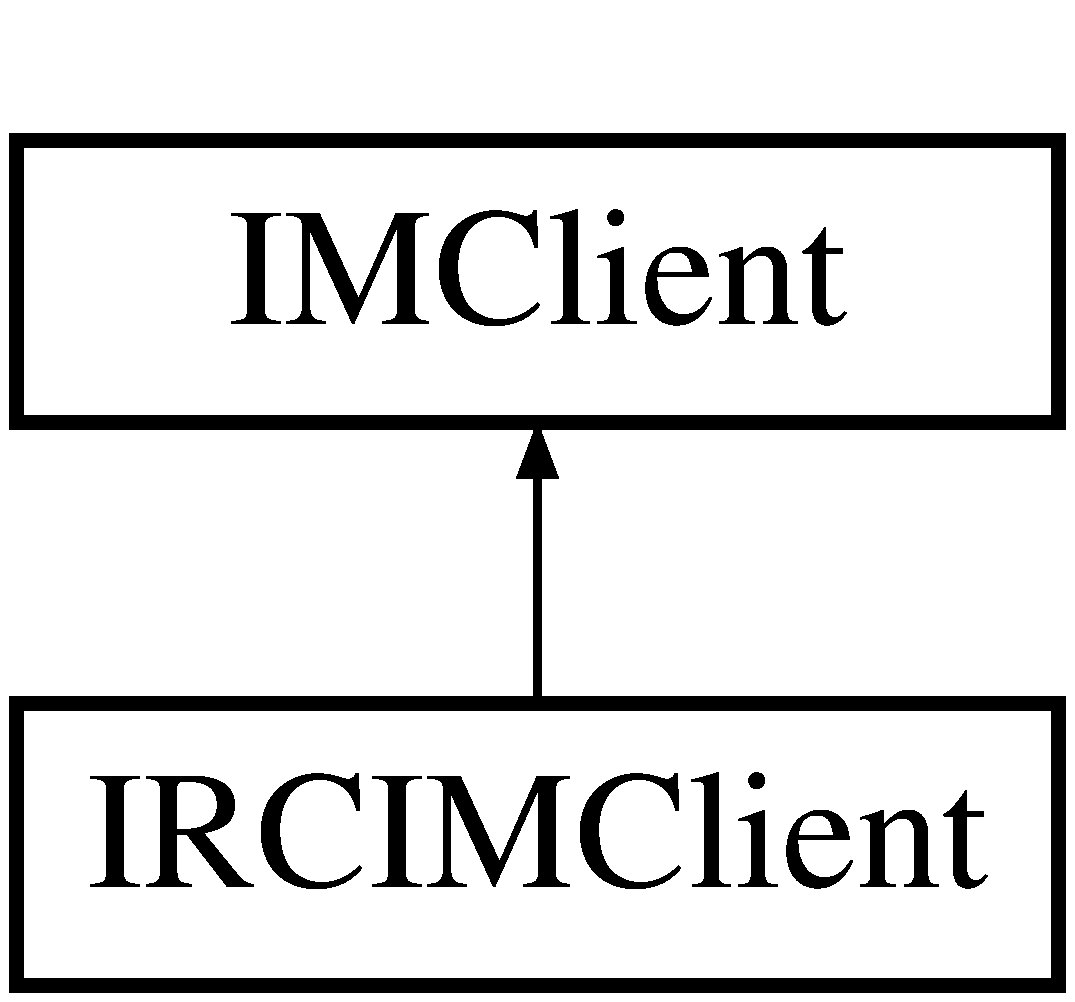
\includegraphics[height=2cm]{classIRCIMClient}
\end{center}
\end{figure}
\subsection*{Signals}
\begin{DoxyCompactItemize}
\item 
\hypertarget{classIRCIMClient_a727c2876a18e56ae354bbdf97d7680ed}{
void {\bfseries connected} ()}
\label{classIRCIMClient_a727c2876a18e56ae354bbdf97d7680ed}

\item 
\hypertarget{classIRCIMClient_a0ccbc2d9556b490b74be7d4b54a94448}{
void {\bfseries disconnected} ()}
\label{classIRCIMClient_a0ccbc2d9556b490b74be7d4b54a94448}

\item 
\hypertarget{classIRCIMClient_a6d5ebb2b5acc008cabcb94fb100e0b60}{
void {\bfseries gotMsg} (QString from, QString message)}
\label{classIRCIMClient_a6d5ebb2b5acc008cabcb94fb100e0b60}

\item 
\hypertarget{classIRCIMClient_a5e87342f449aa6d428318efdb4eb300f}{
void {\bfseries error} (QString errorMsg)}
\label{classIRCIMClient_a5e87342f449aa6d428318efdb4eb300f}

\end{DoxyCompactItemize}
\subsection*{Public Member Functions}
\begin{DoxyCompactItemize}
\item 
\hypertarget{classIRCIMClient_a5205a3ac78186c358f5783e2e258a85c}{
{\bfseries IRCIMClient} (\hyperlink{classIMAccount}{IMAccount} \&account)}
\label{classIRCIMClient_a5205a3ac78186c358f5783e2e258a85c}

\item 
\hypertarget{classIRCIMClient_a4e9046dc26fa3b9a52f098a9910c3ed4}{
void {\bfseries sendMsg} (QString target, QString message)}
\label{classIRCIMClient_a4e9046dc26fa3b9a52f098a9910c3ed4}

\item 
\hypertarget{classIRCIMClient_a9e2ffb96be85534373fb4748d46b99b7}{
QStringList {\bfseries getPresence} ()}
\label{classIRCIMClient_a9e2ffb96be85534373fb4748d46b99b7}

\item 
\hypertarget{classIRCIMClient_aaaa2b995bb752501a68c303b2af5c719}{
void {\bfseries login} ()}
\label{classIRCIMClient_aaaa2b995bb752501a68c303b2af5c719}

\item 
\hypertarget{classIRCIMClient_af6ee63c7d521693111736c344c9472d8}{
void {\bfseries logout} ()}
\label{classIRCIMClient_af6ee63c7d521693111736c344c9472d8}

\item 
\hypertarget{classIRCIMClient_a3a3059e4f284db277fc4d0092cca3b91}{
bool {\bfseries hasUser} (QString user)}
\label{classIRCIMClient_a3a3059e4f284db277fc4d0092cca3b91}

\end{DoxyCompactItemize}


The documentation for this class was generated from the following files:\begin{DoxyCompactItemize}
\item 
adapter/adapter.h\item 
adapter/adapter.cpp\item 
adapter/examples/msg/moc\_\-adapter.cpp\end{DoxyCompactItemize}

\hypertarget{classMd5}{
\section{Md5 Class Reference}
\label{classMd5}\index{Md5@{Md5}}
}
\subsection*{Public Member Functions}
\begin{DoxyCompactItemize}
\item 
\hypertarget{classMd5_a87807ca33ebc9628f15f08cc369942f9}{
{\bfseries Md5} (const void $\ast$input, size\_\-t length)}
\label{classMd5_a87807ca33ebc9628f15f08cc369942f9}

\item 
\hypertarget{classMd5_a29a265f69e72089efb653bd0fa3cfaeb}{
{\bfseries Md5} (const QString \&str)}
\label{classMd5_a29a265f69e72089efb653bd0fa3cfaeb}

\item 
\hypertarget{classMd5_a75fc5c169c898f350bca068bf97e55da}{
void {\bfseries update} (const void $\ast$input, size\_\-t length)}
\label{classMd5_a75fc5c169c898f350bca068bf97e55da}

\item 
\hypertarget{classMd5_af73c5a64419f39914bbb747e92da415a}{
void {\bfseries update} (const QString \&str)}
\label{classMd5_af73c5a64419f39914bbb747e92da415a}

\item 
\hypertarget{classMd5_a40a6af361fdaa7231c75fc0bcc925b41}{
const byte $\ast$ {\bfseries digest} ()}
\label{classMd5_a40a6af361fdaa7231c75fc0bcc925b41}

\item 
\hypertarget{classMd5_ac8a4810328de2b25561d4d3fa7b35018}{
QString {\bfseries toString} ()}
\label{classMd5_ac8a4810328de2b25561d4d3fa7b35018}

\item 
\hypertarget{classMd5_ab5a5e4ddd985062cdae05540ef0b5152}{
void {\bfseries reset} ()}
\label{classMd5_ab5a5e4ddd985062cdae05540ef0b5152}

\end{DoxyCompactItemize}


The documentation for this class was generated from the following files:\begin{DoxyCompactItemize}
\item 
protocols/msn/md5.h\item 
protocols/msn/md5.cpp\end{DoxyCompactItemize}

\hypertarget{classIMFramework_1_1Messenger}{
\section{IMFramework::Messenger Class Reference}
\label{classIMFramework_1_1Messenger}\index{IMFramework::Messenger@{IMFramework::Messenger}}
}
Inheritance diagram for IMFramework::Messenger:\begin{figure}[H]
\begin{center}
\leavevmode
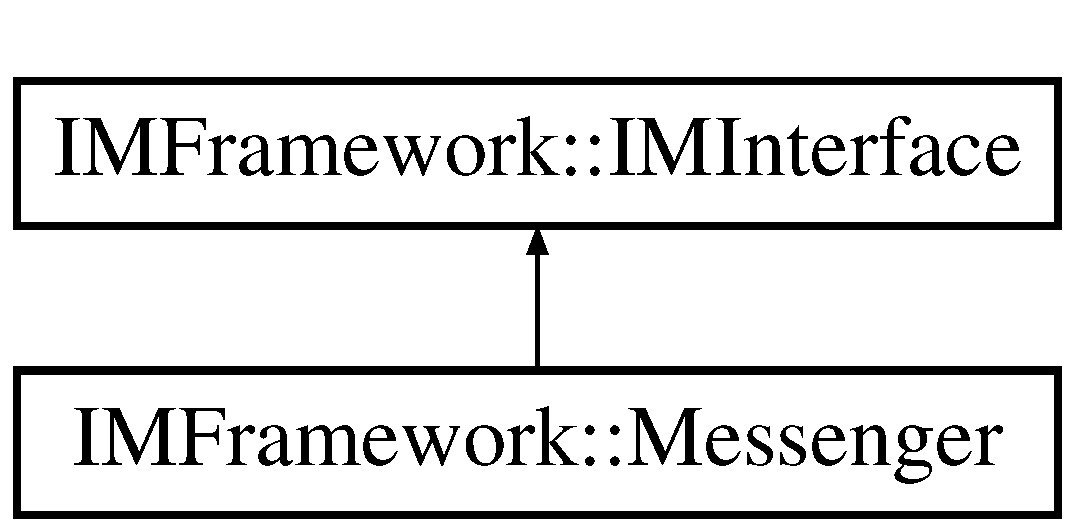
\includegraphics[height=2cm]{classIMFramework_1_1Messenger}
\end{center}
\end{figure}
\subsection*{Public Member Functions}
\begin{DoxyCompactItemize}
\item 
\hypertarget{classIMFramework_1_1Messenger_a60f5e34abab1e90f6a8c60942168db2d}{
{\bfseries Messenger} (QString type)}
\label{classIMFramework_1_1Messenger_a60f5e34abab1e90f6a8c60942168db2d}

\item 
\hypertarget{classIMFramework_1_1Messenger_a0621b125cd33b2e6073a5c48e6a75509}{
long long {\bfseries send} (QVariant msg, QString receiver=\char`\"{}\char`\"{})}
\label{classIMFramework_1_1Messenger_a0621b125cd33b2e6073a5c48e6a75509}

\item 
\hypertarget{classIMFramework_1_1Messenger_a937bfc392b78a9e6524328adaf46a9bb}{
long long {\bfseries send} (QVariant msg, QStringList receiver)}
\label{classIMFramework_1_1Messenger_a937bfc392b78a9e6524328adaf46a9bb}

\item 
\hypertarget{classIMFramework_1_1Messenger_a65dc3f2fa38d187aa5f411e0e27483d9}{
void {\bfseries sendPlainMsg} (QString msg, QString receiver=\char`\"{}\char`\"{})}
\label{classIMFramework_1_1Messenger_a65dc3f2fa38d187aa5f411e0e27483d9}

\end{DoxyCompactItemize}


The documentation for this class was generated from the following files:\begin{DoxyCompactItemize}
\item 
adapter/interface.h\item 
adapter/interface.cpp\end{DoxyCompactItemize}

\hypertarget{classMime}{
\section{Mime Class Reference}
\label{classMime}\index{Mime@{Mime}}
}
\subsection*{Public Member Functions}
\begin{DoxyCompactItemize}
\item 
\hypertarget{classMime_ab46debb17499b419e289776867ec87af}{
{\bfseries Mime} (QString input)}
\label{classMime_ab46debb17499b419e289776867ec87af}

\item 
\hypertarget{classMime_add9a610f058b22d991db70ad231e182d}{
QString {\bfseries getHtml} ()}
\label{classMime_add9a610f058b22d991db70ad231e182d}

\item 
\hypertarget{classMime_ae27161f748bf681a924b9ff536d95942}{
void {\bfseries print} ()}
\label{classMime_ae27161f748bf681a924b9ff536d95942}

\end{DoxyCompactItemize}
\subsection*{Public Attributes}
\begin{DoxyCompactItemize}
\item 
\hypertarget{classMime_a1c7bb9724fe9954cf0c7c745a3be5b25}{
QString {\bfseries payload}}
\label{classMime_a1c7bb9724fe9954cf0c7c745a3be5b25}

\item 
\hypertarget{classMime_ab6c9f29d6d8bd11f639fbabda000c741}{
QString {\bfseries mimeVersion}}
\label{classMime_ab6c9f29d6d8bd11f639fbabda000c741}

\item 
\hypertarget{classMime_ab0c4a695d1fe22acfea55b4f7384f5da}{
QString {\bfseries contentType}}
\label{classMime_ab0c4a695d1fe22acfea55b4f7384f5da}

\item 
\hypertarget{classMime_a2d1ca174d77792ba1bd590eb9498cf7d}{
QString {\bfseries userAgent}}
\label{classMime_a2d1ca174d77792ba1bd590eb9498cf7d}

\item 
\hypertarget{classMime_a4139721fc511240ec60402f4db44a92f}{
QString {\bfseries xMmsImFormat}}
\label{classMime_a4139721fc511240ec60402f4db44a92f}

\item 
\hypertarget{classMime_a75b28ee46d80dc7a5fa67c89a41bced5}{
QString {\bfseries typingUser}}
\label{classMime_a75b28ee46d80dc7a5fa67c89a41bced5}

\item 
\hypertarget{classMime_a449c5711e7419e880e6081f9c669e80f}{
QString {\bfseries font}}
\label{classMime_a449c5711e7419e880e6081f9c669e80f}

\item 
\hypertarget{classMime_a3a8ef272711a0bec1af813d7a5797732}{
QString {\bfseries effect}}
\label{classMime_a3a8ef272711a0bec1af813d7a5797732}

\item 
\hypertarget{classMime_ae32bfaced2d5138538ccbdad9477f726}{
QString {\bfseries color}}
\label{classMime_ae32bfaced2d5138538ccbdad9477f726}

\item 
\hypertarget{classMime_a2817ca6fcdb014fb3523cb9969189b70}{
QString {\bfseries charset}}
\label{classMime_a2817ca6fcdb014fb3523cb9969189b70}

\item 
\hypertarget{classMime_a96cc1d6b32ffcaf046b568271d26fe5d}{
QString {\bfseries pitchAndFamily}}
\label{classMime_a96cc1d6b32ffcaf046b568271d26fe5d}

\end{DoxyCompactItemize}


The documentation for this class was generated from the following file:\begin{DoxyCompactItemize}
\item 
protocols/msn/mime.h\end{DoxyCompactItemize}

\hypertarget{classMsn}{
\section{Msn Class Reference}
\label{classMsn}\index{Msn@{Msn}}
}
\subsection*{Public Slots}
\begin{DoxyCompactItemize}
\item 
\hypertarget{classMsn_ae5b3b36d57ac78ee3f1fab34c93a55cc}{
bool {\bfseries loginMsn} ()}
\label{classMsn_ae5b3b36d57ac78ee3f1fab34c93a55cc}

\item 
\hypertarget{classMsn_ae2204eac2373c0a0064d683e9a75b2a1}{
void {\bfseries removeSB} (\hyperlink{classSwitchBoardSession}{SwitchBoardSession} $\ast$session)}
\label{classMsn_ae2204eac2373c0a0064d683e9a75b2a1}

\end{DoxyCompactItemize}
\subsection*{Signals}
\begin{DoxyCompactItemize}
\item 
\hypertarget{classMsn_aba018794aa94476d447765c836c6c69d}{
void {\bfseries msgReceived} (QString message, QString sender, \hyperlink{classSwitchBoardSession}{SwitchBoardSession} $\ast$session)}
\label{classMsn_aba018794aa94476d447765c836c6c69d}

\item 
\hypertarget{classMsn_ae53ae3b871d26efefb840ea42e8c90a1}{
void {\bfseries rawMsgReceived} (QString message, QString sender, \hyperlink{classSwitchBoardSession}{SwitchBoardSession} $\ast$session)}
\label{classMsn_ae53ae3b871d26efefb840ea42e8c90a1}

\item 
\hypertarget{classMsn_a8b6cb40cb5b089087fca2143f46bf512}{
void {\bfseries invitedToSession} (\hyperlink{classMsnContact}{MsnContact} invitor, \hyperlink{classSwitchBoardSession}{SwitchBoardSession} $\ast$session)}
\label{classMsn_a8b6cb40cb5b089087fca2143f46bf512}

\item 
\hypertarget{classMsn_a5980c33d1c9d5f41b7b7a9b355ed966a}{
void {\bfseries contactOnline} (\hyperlink{classMsnContact}{MsnContact} contact)}
\label{classMsn_a5980c33d1c9d5f41b7b7a9b355ed966a}

\item 
\hypertarget{classMsn_aa8425b196e9f19493a1413a924883d25}{
void {\bfseries contactOffline} (\hyperlink{classMsnContact}{MsnContact} contact)}
\label{classMsn_aa8425b196e9f19493a1413a924883d25}

\item 
\hypertarget{classMsn_a5473c5582f65220fae3f068aed91332e}{
void {\bfseries contactStatusChanged} (\hyperlink{classMsnContact}{MsnContact} contact, QString status)}
\label{classMsn_a5473c5582f65220fae3f068aed91332e}

\item 
\hypertarget{classMsn_aed7345010e54e133b6f8c74ae5aaaa98}{
void {\bfseries beingAddedBy} (\hyperlink{classMsnContact}{MsnContact} contact)}
\label{classMsn_aed7345010e54e133b6f8c74ae5aaaa98}

\item 
\hypertarget{classMsn_a0b7ff4e1ea5ba0ed522dbaffc681c928}{
void {\bfseries userJoinSession} (\hyperlink{classSwitchBoardSession}{SwitchBoardSession} $\ast$sb, QString email)}
\label{classMsn_a0b7ff4e1ea5ba0ed522dbaffc681c928}

\item 
\hypertarget{classMsn_a9a2568f2b5308fad5bbdfcbb97c55c5a}{
void {\bfseries userLeftSession} (\hyperlink{classSwitchBoardSession}{SwitchBoardSession} $\ast$sb, QString email)}
\label{classMsn_a9a2568f2b5308fad5bbdfcbb97c55c5a}

\item 
\hypertarget{classMsn_af2b3d9a81e0b2b5b8e25e7492e17deb1}{
void {\bfseries loginFinish} ()}
\label{classMsn_af2b3d9a81e0b2b5b8e25e7492e17deb1}

\item 
\hypertarget{classMsn_a8a40e2fbfd9778cfad9ea90518378b7f}{
void {\bfseries syncSession} ()}
\label{classMsn_a8a40e2fbfd9778cfad9ea90518378b7f}

\item 
\hypertarget{classMsn_adb9fe086f63745ccde55ee68bb4ac8f7}{
void {\bfseries contactListChanged} ()}
\label{classMsn_adb9fe086f63745ccde55ee68bb4ac8f7}

\item 
\hypertarget{classMsn_a5170af24615e113721c74f411f8a26bd}{
void {\bfseries userTyping} (QString email)}
\label{classMsn_a5170af24615e113721c74f411f8a26bd}

\item 
\hypertarget{classMsn_a7666637d86bb1ded43677d2d6659218b}{
void {\bfseries sessionTyping} (\hyperlink{classSwitchBoardSession}{SwitchBoardSession} $\ast$sb)}
\label{classMsn_a7666637d86bb1ded43677d2d6659218b}

\end{DoxyCompactItemize}
\subsection*{Public Member Functions}
\begin{DoxyCompactItemize}
\item 
\hypertarget{classMsn_aae02bad6846b3aff0753a57d04046ca4}{
void {\bfseries setUsernamePassword} (QString username, QString password)}
\label{classMsn_aae02bad6846b3aff0753a57d04046ca4}

\item 
\hypertarget{classMsn_a721ff6d8bbec8fec1ea1f57cbf0ab2d0}{
void {\bfseries setStatus} (QString status)}
\label{classMsn_a721ff6d8bbec8fec1ea1f57cbf0ab2d0}

\item 
\hypertarget{classMsn_a20f729ae9af9b6a0635233793290da82}{
void {\bfseries sendMsg} (QString receiver, QString message)}
\label{classMsn_a20f729ae9af9b6a0635233793290da82}

\item 
\hypertarget{classMsn_ae6bad5afb2a66233a86e3e24c944c5d9}{
void {\bfseries addContact} (QString contact, QString group)}
\label{classMsn_ae6bad5afb2a66233a86e3e24c944c5d9}

\item 
\hypertarget{classMsn_a98ba30441700908d47ba797396d510cc}{
void {\bfseries removeContact} (QString contact)}
\label{classMsn_a98ba30441700908d47ba797396d510cc}

\item 
\hypertarget{classMsn_aa9d0b35905dd05487873e3232b91f98d}{
void {\bfseries blockContact} (QString contact)}
\label{classMsn_aa9d0b35905dd05487873e3232b91f98d}

\item 
\hypertarget{classMsn_a32813babfc06cfd8bbaaa1c7efa77acc}{
void {\bfseries unblockContact} (QString contact)}
\label{classMsn_a32813babfc06cfd8bbaaa1c7efa77acc}

\item 
\hypertarget{classMsn_a802bf36e77f75e53e29a5cf4e9b2a5c6}{
QMap$<$ QString, QString $>$ {\bfseries getProfile} (\hyperlink{classMsnContact}{MsnContact} contact)}
\label{classMsn_a802bf36e77f75e53e29a5cf4e9b2a5c6}

\item 
\hypertarget{classMsn_ab13250da6eae22c6a489cefadad474c5}{
QList$<$ \hyperlink{classMsnContact}{MsnContact} $\ast$ $>$ {\bfseries getContacts} (QString status)}
\label{classMsn_ab13250da6eae22c6a489cefadad474c5}

\item 
\hypertarget{classMsn_a07015e42deec5bf5c2d8666e6e43ccd0}{
QList$<$ QString $>$ {\bfseries getContactsEmails} (QString status)}
\label{classMsn_a07015e42deec5bf5c2d8666e6e43ccd0}

\item 
\hypertarget{classMsn_a12913a2f65c8d7eb15179712aaef5c2d}{
\hyperlink{classSwitchBoardSession}{SwitchBoardSession} $\ast$ {\bfseries requestSBSession} (QString receiver)}
\label{classMsn_a12913a2f65c8d7eb15179712aaef5c2d}

\item 
\hypertarget{classMsn_a7e3bba3d88bb937b2c18daf59a939a38}{
\hyperlink{classMsnContact}{MsnContact} $\ast$ {\bfseries findContact} (QString type, QString value)}
\label{classMsn_a7e3bba3d88bb937b2c18daf59a939a38}

\end{DoxyCompactItemize}
\subsection*{Public Attributes}
\begin{DoxyCompactItemize}
\item 
\hypertarget{classMsn_a0802edd087139a66586fbdfdf1087c9f}{
QList$<$ \hyperlink{classSwitchBoardSession}{SwitchBoardSession} $\ast$ $>$ {\bfseries m\_\-sessions}}
\label{classMsn_a0802edd087139a66586fbdfdf1087c9f}

\end{DoxyCompactItemize}


The documentation for this class was generated from the following files:\begin{DoxyCompactItemize}
\item 
protocols/msn/msn.h\item 
protocols/msn/msn.cpp\end{DoxyCompactItemize}

\hypertarget{classMsnAuth}{
\section{MsnAuth Class Reference}
\label{classMsnAuth}\index{MsnAuth@{MsnAuth}}
}
\subsection*{Signals}
\begin{DoxyCompactItemize}
\item 
\hypertarget{classMsnAuth_a272dd22c96b336a1f97362c4309b6a8b}{
void {\bfseries authCompleted} (QString authenticationString)}
\label{classMsnAuth_a272dd22c96b336a1f97362c4309b6a8b}

\end{DoxyCompactItemize}
\subsection*{Public Member Functions}
\begin{DoxyCompactItemize}
\item 
\hypertarget{classMsnAuth_ab7b086e29a4624cea5459d7a8b4e34fa}{
{\bfseries MsnAuth} (QString userName, QString password, QString ticket)}
\label{classMsnAuth_ab7b086e29a4624cea5459d7a8b4e34fa}

\item 
\hypertarget{classMsnAuth_ac28a69b24c4443018ddcd7c60a9efb73}{
void {\bfseries authenticate} ()}
\label{classMsnAuth_ac28a69b24c4443018ddcd7c60a9efb73}

\end{DoxyCompactItemize}


The documentation for this class was generated from the following files:\begin{DoxyCompactItemize}
\item 
protocols/msn/msnauth.h\item 
protocols/msn/msnauth.cpp\end{DoxyCompactItemize}

\hypertarget{classMsnChallenge}{
\section{MsnChallenge Class Reference}
\label{classMsnChallenge}\index{MsnChallenge@{MsnChallenge}}
}
\subsection*{Public Member Functions}
\begin{DoxyCompactItemize}
\item 
\hypertarget{classMsnChallenge_ababd5054592f2eac6ddbe5a47dbc25af}{
{\bfseries MsnChallenge} (QString pId, QString pKey)}
\label{classMsnChallenge_ababd5054592f2eac6ddbe5a47dbc25af}

\item 
\hypertarget{classMsnChallenge_ab5c244a5881cf3e4179dad2e3d0f6072}{
QString {\bfseries calculateChallenge} (QString input)}
\label{classMsnChallenge_ab5c244a5881cf3e4179dad2e3d0f6072}

\end{DoxyCompactItemize}


The documentation for this class was generated from the following file:\begin{DoxyCompactItemize}
\item 
protocols/msn/challenge.h\end{DoxyCompactItemize}

\hypertarget{classMsnContact}{
\section{MsnContact Class Reference}
\label{classMsnContact}\index{MsnContact@{MsnContact}}
}
\subsection*{Public Member Functions}
\begin{DoxyCompactItemize}
\item 
\hypertarget{classMsnContact_a00ac0df3e7a006c09e4d9359109e745a}{
bool {\bfseries set} (QString pName, QString pValue)}
\label{classMsnContact_a00ac0df3e7a006c09e4d9359109e745a}

\item 
\hypertarget{classMsnContact_ae0a8d5af118d4cd4563faf0172d63c49}{
QString {\bfseries get} (QString pName)}
\label{classMsnContact_ae0a8d5af118d4cd4563faf0172d63c49}

\item 
\hypertarget{classMsnContact_adfd76fa3929a48471aa90e6e25833f36}{
bool {\bfseries delProperty} (QString pName)}
\label{classMsnContact_adfd76fa3929a48471aa90e6e25833f36}

\item 
\hypertarget{classMsnContact_a0f0a7369cde876bd2e8e5fa89bc47888}{
void {\bfseries print} ()}
\label{classMsnContact_a0f0a7369cde876bd2e8e5fa89bc47888}

\item 
\hypertarget{classMsnContact_af4e22680ec4504831d0f98f1b2f48630}{
QString {\bfseries toString} ()}
\label{classMsnContact_af4e22680ec4504831d0f98f1b2f48630}

\end{DoxyCompactItemize}


The documentation for this class was generated from the following file:\begin{DoxyCompactItemize}
\item 
protocols/msn/msncontact.h\end{DoxyCompactItemize}

\hypertarget{classMsnContactList}{
\section{MsnContactList Class Reference}
\label{classMsnContactList}\index{MsnContactList@{MsnContactList}}
}
\subsection*{Signals}
\begin{DoxyCompactItemize}
\item 
\hypertarget{classMsnContactList_a9ccc8f8b3eddd028c8e78fbdd7de3b78}{
void {\bfseries gotBuddyList} ()}
\label{classMsnContactList_a9ccc8f8b3eddd028c8e78fbdd7de3b78}

\end{DoxyCompactItemize}
\subsection*{Public Member Functions}
\begin{DoxyCompactItemize}
\item 
\hypertarget{classMsnContactList_af39ccd3a758122f876c554c70d65c7d2}{
{\bfseries MsnContactList} (QString mspAuth)}
\label{classMsnContactList_af39ccd3a758122f876c554c70d65c7d2}

\item 
\hypertarget{classMsnContactList_af1adeb6e8c5e65a6a56af9e8d60a6a07}{
bool {\bfseries requestMembershipList} ()}
\label{classMsnContactList_af1adeb6e8c5e65a6a56af9e8d60a6a07}

\item 
\hypertarget{classMsnContactList_aa9e3b1fe5b3cabbe4b1faba6334595e0}{
bool {\bfseries requestAddressBook} ()}
\label{classMsnContactList_aa9e3b1fe5b3cabbe4b1faba6334595e0}

\item 
\hypertarget{classMsnContactList_a7ce58fd287ee7b634f8a04bdb66ca2d4}{
QString {\bfseries ml} ()}
\label{classMsnContactList_a7ce58fd287ee7b634f8a04bdb66ca2d4}

\end{DoxyCompactItemize}


The documentation for this class was generated from the following files:\begin{DoxyCompactItemize}
\item 
protocols/msn/contactlist.h\item 
protocols/msn/contactlist.cpp\end{DoxyCompactItemize}

\hypertarget{classMsnSession}{
\section{MsnSession Class Reference}
\label{classMsnSession}\index{MsnSession@{MsnSession}}
}
\subsection*{Signals}
\begin{DoxyCompactItemize}
\item 
\hypertarget{classMsnSession_a5abea6a694eb03afe3b4a6fac8af884b}{
void {\bfseries incomingMsg} (QString answer)}
\label{classMsnSession_a5abea6a694eb03afe3b4a6fac8af884b}

\item 
\hypertarget{classMsnSession_ad60cd76fc8b3cadeb622888ec34f01e4}{
void {\bfseries disconnected} ()}
\label{classMsnSession_ad60cd76fc8b3cadeb622888ec34f01e4}

\end{DoxyCompactItemize}
\subsection*{Public Member Functions}
\begin{DoxyCompactItemize}
\item 
\hypertarget{classMsnSession_a30e08ba72966421aadad02e09d7df5f1}{
{\bfseries MsnSession} (QString server, int port)}
\label{classMsnSession_a30e08ba72966421aadad02e09d7df5f1}

\item 
\hypertarget{classMsnSession_ac0df2e2acb33aba75c8c4870812574bf}{
{\bfseries MsnSession} (QString serverAndPort)}
\label{classMsnSession_ac0df2e2acb33aba75c8c4870812574bf}

\item 
\hypertarget{classMsnSession_a1bdac5fcf73924a3c81d3e34ac5fe7b8}{
int {\bfseries sendCommand} (const char $\ast$cmd, QString p1=\char`\"{}\char`\"{}, QString p2=\char`\"{}\char`\"{}, QString p3=\char`\"{}\char`\"{}, QString p4=\char`\"{}\char`\"{})}
\label{classMsnSession_a1bdac5fcf73924a3c81d3e34ac5fe7b8}

\item 
\hypertarget{classMsnSession_aa6f156e3c5a7dbc76e735b1a6bceca97}{
QString {\bfseries sendAndWait} (const char $\ast$cmd, QString p1=\char`\"{}\char`\"{}, QString p2=\char`\"{}\char`\"{}, QString p3=\char`\"{}\char`\"{}, QString p4=\char`\"{}\char`\"{})}
\label{classMsnSession_aa6f156e3c5a7dbc76e735b1a6bceca97}

\item 
\hypertarget{classMsnSession_aa3562f72464aa050480b74bb7083a98b}{
QString {\bfseries getAnswer} (int cmdIndex, int timeOut=2000)}
\label{classMsnSession_aa3562f72464aa050480b74bb7083a98b}

\item 
\hypertarget{classMsnSession_a82a9d08f3a777c698c45d44130c03ebe}{
QString {\bfseries findReg} (QString regExp, QString findIn, int whichText)}
\label{classMsnSession_a82a9d08f3a777c698c45d44130c03ebe}

\item 
\hypertarget{classMsnSession_a7aa744964796a46be39f673ceb396871}{
int {\bfseries state} ()}
\label{classMsnSession_a7aa744964796a46be39f673ceb396871}

\end{DoxyCompactItemize}
\subsection*{Public Attributes}
\begin{DoxyCompactItemize}
\item 
\hypertarget{classMsnSession_a80b2bf50002a8852bd6526244e237a6c}{
QString {\bfseries mspAuth}}
\label{classMsnSession_a80b2bf50002a8852bd6526244e237a6c}

\end{DoxyCompactItemize}


The documentation for this class was generated from the following files:\begin{DoxyCompactItemize}
\item 
protocols/msn/msnsession.h\item 
protocols/msn/msnsession.cpp\end{DoxyCompactItemize}

\hypertarget{classIMFramework_1_1Presence}{
\section{IMFramework::Presence Class Reference}
\label{classIMFramework_1_1Presence}\index{IMFramework::Presence@{IMFramework::Presence}}
}
Inheritance diagram for IMFramework::Presence:\begin{figure}[H]
\begin{center}
\leavevmode
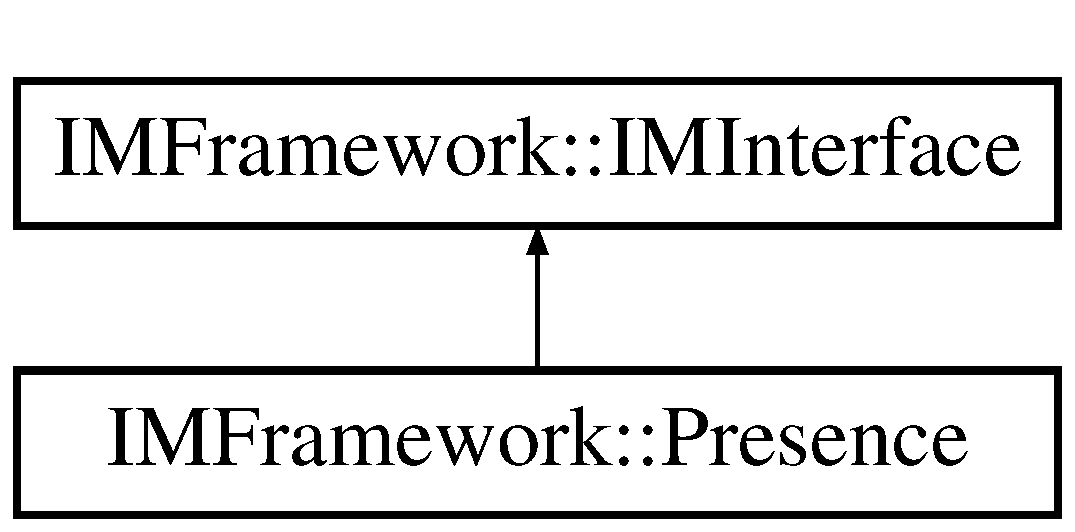
\includegraphics[height=2cm]{classIMFramework_1_1Presence}
\end{center}
\end{figure}
\subsection*{Signals}
\begin{DoxyCompactItemize}
\item 
\hypertarget{classIMFramework_1_1Presence_a01d5e8d5a517819fbdb358815109deb8}{
void {\bfseries presenceChanged} (QString buddy, QString status)}
\label{classIMFramework_1_1Presence_a01d5e8d5a517819fbdb358815109deb8}

\item 
\hypertarget{classIMFramework_1_1Presence_a59e2222d3f2c1d3e5356e6c7b448ece3}{
void {\bfseries updated} ()}
\label{classIMFramework_1_1Presence_a59e2222d3f2c1d3e5356e6c7b448ece3}

\end{DoxyCompactItemize}
\subsection*{Public Member Functions}
\begin{DoxyCompactItemize}
\item 
\hypertarget{classIMFramework_1_1Presence_ab5babc9cd970b23b5dfcc716e221d923}{
QString {\bfseries getPresence} (QString buddy)}
\label{classIMFramework_1_1Presence_ab5babc9cd970b23b5dfcc716e221d923}

\item 
\hypertarget{classIMFramework_1_1Presence_adf265d6547d736cb764d9597b707daf9}{
void {\bfseries monitor} (QString buddy, bool subscribe=true)}
\label{classIMFramework_1_1Presence_adf265d6547d736cb764d9597b707daf9}

\item 
\hypertarget{classIMFramework_1_1Presence_a06e4622508dccda11049c6e9f214b037}{
QStringList {\bfseries allOnline} ()}
\label{classIMFramework_1_1Presence_a06e4622508dccda11049c6e9f214b037}

\end{DoxyCompactItemize}
\subsection*{Protected Slots}
\begin{DoxyCompactItemize}
\item 
\hypertarget{classIMFramework_1_1Presence_ab219d4d88b2b0ba5d7740138e8f350e2}{
virtual void {\bfseries gotMsg} (QString from, QString dest, QString msg, long long replyTo)}
\label{classIMFramework_1_1Presence_ab219d4d88b2b0ba5d7740138e8f350e2}

\end{DoxyCompactItemize}


The documentation for this class was generated from the following files:\begin{DoxyCompactItemize}
\item 
adapter/interface.h\item 
adapter/examples/msg/moc\_\-interface.cpp\item 
adapter/interface.cpp\end{DoxyCompactItemize}

\hypertarget{classIMFramework_1_1Query}{
\section{IMFramework::Query Class Reference}
\label{classIMFramework_1_1Query}\index{IMFramework::Query@{IMFramework::Query}}
}
Inheritance diagram for IMFramework::Query:\begin{figure}[H]
\begin{center}
\leavevmode
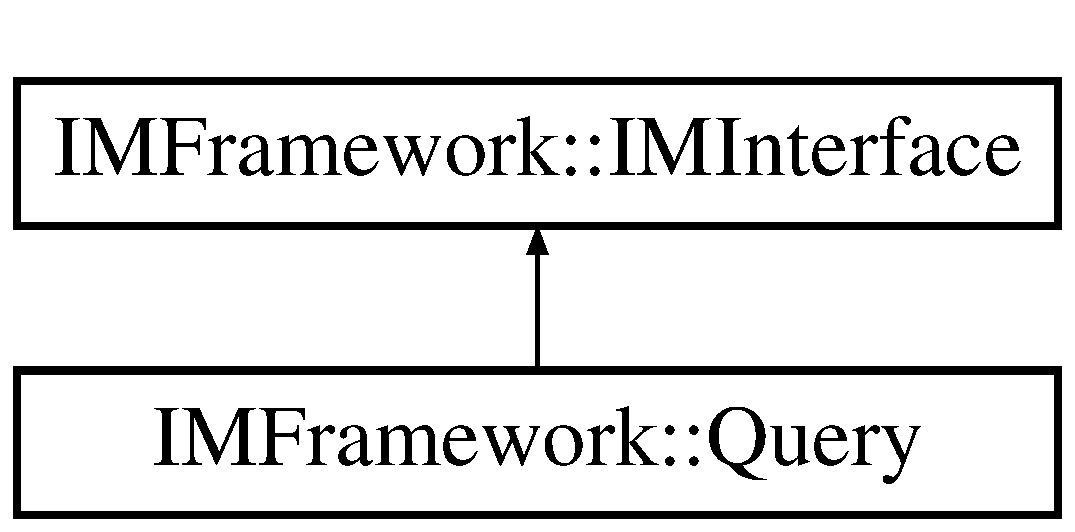
\includegraphics[height=2cm]{classIMFramework_1_1Query}
\end{center}
\end{figure}
\subsection*{Signals}
\begin{DoxyCompactItemize}
\item 
\hypertarget{classIMFramework_1_1Query_ae3523e46600c76138027d3cf4e663a4d}{
void {\bfseries reply} (QVariant result, long long answerTo, QString fromServer)}
\label{classIMFramework_1_1Query_ae3523e46600c76138027d3cf4e663a4d}

\end{DoxyCompactItemize}
\subsection*{Public Member Functions}
\begin{DoxyCompactItemize}
\item 
\hypertarget{classIMFramework_1_1Query_aa35bfaeeb38a1b64aaeff6d8f07e45eb}{
long long {\bfseries ask} (QVariant query, QString preferableFormat)}
\label{classIMFramework_1_1Query_aa35bfaeeb38a1b64aaeff6d8f07e45eb}

\end{DoxyCompactItemize}


The documentation for this class was generated from the following files:\begin{DoxyCompactItemize}
\item 
adapter/interface.h\item 
adapter/examples/msg/moc\_\-interface.cpp\end{DoxyCompactItemize}

\hypertarget{classQuerySender}{
\section{QuerySender Class Reference}
\label{classQuerySender}\index{QuerySender@{QuerySender}}
}
\subsection*{Signals}
\begin{DoxyCompactItemize}
\item 
\hypertarget{classQuerySender_ae0295b63e8c81d285f83f152db5fe724}{
void {\bfseries getAnswer} (Group from, QVariant results)}
\label{classQuerySender_ae0295b63e8c81d285f83f152db5fe724}

\end{DoxyCompactItemize}
\subsection*{Public Member Functions}
\begin{DoxyCompactItemize}
\item 
\hypertarget{classQuerySender_a1c70fd551a21aaff8dbecdb4d2f2aee2}{
void {\bfseries linkTo} (Group server)}
\label{classQuerySender_a1c70fd551a21aaff8dbecdb4d2f2aee2}

\item 
\hypertarget{classQuerySender_a26e94e0a8f9d3db13f3e4246441ccac6}{
void {\bfseries query} (QString sqlQuery, QString format=\char`\"{}\char`\"{})}
\label{classQuerySender_a26e94e0a8f9d3db13f3e4246441ccac6}

\end{DoxyCompactItemize}


The documentation for this class was generated from the following file:\begin{DoxyCompactItemize}
\item 
adapter/examples/query/exam3.h\end{DoxyCompactItemize}

\hypertarget{classQueryServer}{
\section{QueryServer Class Reference}
\label{classQueryServer}\index{QueryServer@{QueryServer}}
}
\subsection*{Public Slots}
\begin{DoxyCompactItemize}
\item 
\hypertarget{classQueryServer_aa3ee87750f7d7effc64c9798ba1ddebd}{
void {\bfseries gotQuery} (QString sqlQuery, QString format)}
\label{classQueryServer_aa3ee87750f7d7effc64c9798ba1ddebd}

\end{DoxyCompactItemize}


The documentation for this class was generated from the following file:\begin{DoxyCompactItemize}
\item 
adapter/examples/query/exam3.h\end{DoxyCompactItemize}

\hypertarget{classSwitchBoardSession}{
\section{SwitchBoardSession Class Reference}
\label{classSwitchBoardSession}\index{SwitchBoardSession@{SwitchBoardSession}}
}
\subsection*{Signals}
\begin{DoxyCompactItemize}
\item 
\hypertarget{classSwitchBoardSession_ac75df6142c80d4bfb174e88647aedc8e}{
void {\bfseries receivedMsg} (QString fromUser, QString fromNick, QString payloadLength, QString payloadBody)}
\label{classSwitchBoardSession_ac75df6142c80d4bfb174e88647aedc8e}

\item 
\hypertarget{classSwitchBoardSession_a0dceadd5add55c20c5e7c2f7e50dc643}{
void {\bfseries leftConversation} (\hyperlink{classSwitchBoardSession}{SwitchBoardSession} $\ast$sb, QString user, QString reason)}
\label{classSwitchBoardSession_a0dceadd5add55c20c5e7c2f7e50dc643}

\item 
\hypertarget{classSwitchBoardSession_a96070e15ac93e28979db4b117836b257}{
void {\bfseries joinConversation} (\hyperlink{classSwitchBoardSession}{SwitchBoardSession} $\ast$sb, QString user, QString reason)}
\label{classSwitchBoardSession_a96070e15ac93e28979db4b117836b257}

\item 
\hypertarget{classSwitchBoardSession_a6b97071275dc16e5943683ad891a9f24}{
void {\bfseries closed} (\hyperlink{classSwitchBoardSession}{SwitchBoardSession} $\ast$me)}
\label{classSwitchBoardSession_a6b97071275dc16e5943683ad891a9f24}

\item 
\hypertarget{classSwitchBoardSession_accc8ca9cb1c11b3aa2757f5a42fe9273}{
void {\bfseries msgReceived} (QString message, QString sender, \hyperlink{classSwitchBoardSession}{SwitchBoardSession} $\ast$session)}
\label{classSwitchBoardSession_accc8ca9cb1c11b3aa2757f5a42fe9273}

\item 
\hypertarget{classSwitchBoardSession_a5e905afb24ad7932e8bdd024ee452f16}{
void {\bfseries rawMsgReceived} (QString message, QString sender, \hyperlink{classSwitchBoardSession}{SwitchBoardSession} $\ast$session)}
\label{classSwitchBoardSession_a5e905afb24ad7932e8bdd024ee452f16}

\item 
\hypertarget{classSwitchBoardSession_a31c5d704ce939c36a5f5466e33d971c6}{
void {\bfseries userTyping} (QString user)}
\label{classSwitchBoardSession_a31c5d704ce939c36a5f5466e33d971c6}

\item 
\hypertarget{classSwitchBoardSession_a7b540933b18c17204f18e8b227402351}{
void {\bfseries sessionTyping} (\hyperlink{classSwitchBoardSession}{SwitchBoardSession} $\ast$sb)}
\label{classSwitchBoardSession_a7b540933b18c17204f18e8b227402351}

\end{DoxyCompactItemize}
\subsection*{Public Member Functions}
\begin{DoxyCompactItemize}
\item 
\hypertarget{classSwitchBoardSession_aa54467cc9f5d064a69811c3a4154b16c}{
{\bfseries SwitchBoardSession} (QStringList oldHistory, QString username, QString invitationCmd)}
\label{classSwitchBoardSession_aa54467cc9f5d064a69811c3a4154b16c}

\item 
\hypertarget{classSwitchBoardSession_a534b510235d697ceafada3974dcfa857}{
{\bfseries SwitchBoardSession} (\hyperlink{classMsnSession}{MsnSession} $\ast$loginSession, QStringList receivers)}
\label{classSwitchBoardSession_a534b510235d697ceafada3974dcfa857}

\item 
\hypertarget{classSwitchBoardSession_a7f73fbeb8b9b45d2772afeb6b3cb5b73}{
bool {\bfseries inviteToThisSession} (QString email)}
\label{classSwitchBoardSession_a7f73fbeb8b9b45d2772afeb6b3cb5b73}

\item 
\hypertarget{classSwitchBoardSession_a9ca703d0ab2ec0dcae5a8470956a87cb}{
void {\bfseries sendMessage} (QString receiver, QString message)}
\label{classSwitchBoardSession_a9ca703d0ab2ec0dcae5a8470956a87cb}

\item 
\hypertarget{classSwitchBoardSession_a9c1425df82566eafe57309c7d3e47093}{
bool {\bfseries talkingTo} (QString email)}
\label{classSwitchBoardSession_a9c1425df82566eafe57309c7d3e47093}

\item 
\hypertarget{classSwitchBoardSession_a719f587f8b2513b230b2b84949a5e040}{
QString {\bfseries getHistory} (int lineCount=10)}
\label{classSwitchBoardSession_a719f587f8b2513b230b2b84949a5e040}

\item 
\hypertarget{classSwitchBoardSession_a6ef53d9017746e9a30161577c6323bf6}{
QString {\bfseries getParticipants} (int desiredLength, \hyperlink{classMsn}{Msn} $\ast$msn)}
\label{classSwitchBoardSession_a6ef53d9017746e9a30161577c6323bf6}

\item 
\hypertarget{classSwitchBoardSession_afc5f702d461af16fb670ddea68552f21}{
void {\bfseries reConnect} ()}
\label{classSwitchBoardSession_afc5f702d461af16fb670ddea68552f21}

\item 
\hypertarget{classSwitchBoardSession_a865139408af38ed43cee1a572d5749fc}{
QStringList {\bfseries allParticipants} ()}
\label{classSwitchBoardSession_a865139408af38ed43cee1a572d5749fc}

\end{DoxyCompactItemize}
\subsection*{Static Public Member Functions}
\begin{DoxyCompactItemize}
\item 
\hypertarget{classSwitchBoardSession_ad0b0421ed84df42ab33488a00ee752a8}{
static QString {\bfseries toShort} (QString input, int length)}
\label{classSwitchBoardSession_ad0b0421ed84df42ab33488a00ee752a8}

\end{DoxyCompactItemize}
\subsection*{Public Attributes}
\begin{DoxyCompactItemize}
\item 
\hypertarget{classSwitchBoardSession_ae3af3477e30a0b1c93424fb397a2f653}{
QStringList {\bfseries m\_\-history}}
\label{classSwitchBoardSession_ae3af3477e30a0b1c93424fb397a2f653}

\end{DoxyCompactItemize}


The documentation for this class was generated from the following files:\begin{DoxyCompactItemize}
\item 
protocols/msn/switchboard.h\item 
protocols/msn/switchboard.cpp\end{DoxyCompactItemize}

\hypertarget{classIMFramework_1_1Synchronizor}{
\section{IMFramework::Synchronizor Class Reference}
\label{classIMFramework_1_1Synchronizor}\index{IMFramework::Synchronizor@{IMFramework::Synchronizor}}
}
Inheritance diagram for IMFramework::Synchronizor:\begin{figure}[H]
\begin{center}
\leavevmode
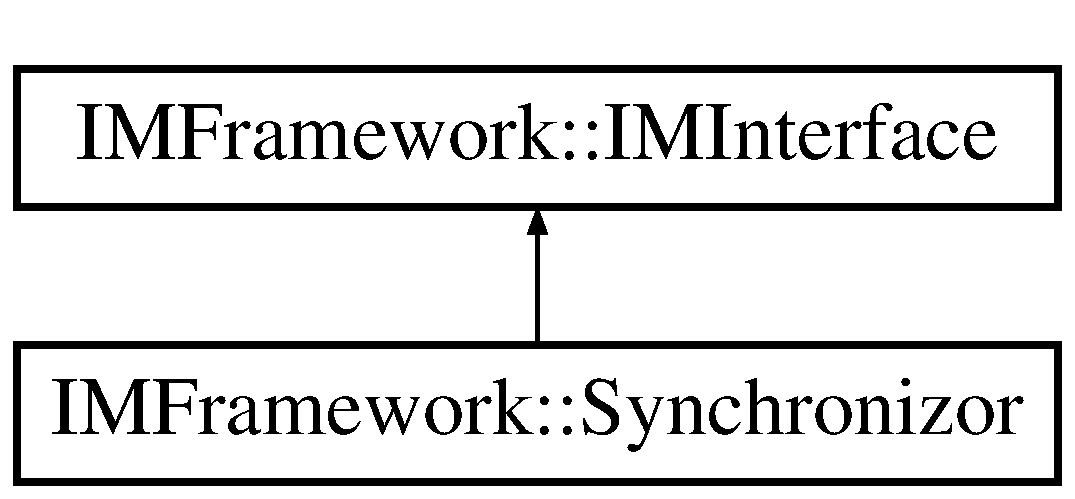
\includegraphics[height=2cm]{classIMFramework_1_1Synchronizor}
\end{center}
\end{figure}
\subsection*{Signals}
\begin{DoxyCompactItemize}
\item 
\hypertarget{classIMFramework_1_1Synchronizor_a1c3990c174267237d7c19bd7cffcc50f}{
void {\bfseries updateFull} (QVariant data)}
\label{classIMFramework_1_1Synchronizor_a1c3990c174267237d7c19bd7cffcc50f}

\end{DoxyCompactItemize}
\subsection*{Public Member Functions}
\begin{DoxyCompactItemize}
\item 
\hypertarget{classIMFramework_1_1Synchronizor_a126cbe0569ad3450ff76d689e0e54740}{
{\bfseries Synchronizor} (QStringList syncWith=QStringList())}
\label{classIMFramework_1_1Synchronizor_a126cbe0569ad3450ff76d689e0e54740}

\item 
\hypertarget{classIMFramework_1_1Synchronizor_a0dc8019a8ea761e238dfc9253e77a667}{
void {\bfseries pushFull} (QVariant data, QStringList toDest=QStringList())}
\label{classIMFramework_1_1Synchronizor_a0dc8019a8ea761e238dfc9253e77a667}

\end{DoxyCompactItemize}


The documentation for this class was generated from the following files:\begin{DoxyCompactItemize}
\item 
adapter/interface.h\item 
adapter/interface.cpp\end{DoxyCompactItemize}

\hypertarget{classSyncTextBox}{
\section{SyncTextBox Class Reference}
\label{classSyncTextBox}\index{SyncTextBox@{SyncTextBox}}
}
\subsection*{Public Slots}
\begin{DoxyCompactItemize}
\item 
\hypertarget{classSyncTextBox_a70e5abaa925d7bd3f344156b69182544}{
void {\bfseries textTyped} ()}
\label{classSyncTextBox_a70e5abaa925d7bd3f344156b69182544}

\item 
\hypertarget{classSyncTextBox_a405d0b6c581451ff8e84c489a4434ac2}{
void {\bfseries textUpdated} ()}
\label{classSyncTextBox_a405d0b6c581451ff8e84c489a4434ac2}

\end{DoxyCompactItemize}
\subsection*{Public Member Functions}
\begin{DoxyCompactItemize}
\item 
\hypertarget{classSyncTextBox_adeb5c3586b4cf3264be225bdbd38d693}{
QString {\bfseries toString} ()}
\label{classSyncTextBox_adeb5c3586b4cf3264be225bdbd38d693}

\item 
\hypertarget{classSyncTextBox_a80a91c980a25feabc57523fcdd0476a9}{
void {\bfseries fromString} ()}
\label{classSyncTextBox_a80a91c980a25feabc57523fcdd0476a9}

\item 
\hypertarget{classSyncTextBox_a640ce6462b534c9c639a837fa1c375ff}{
void {\bfseries syncTo} (Group grp)}
\label{classSyncTextBox_a640ce6462b534c9c639a837fa1c375ff}

\end{DoxyCompactItemize}


The documentation for this class was generated from the following files:\begin{DoxyCompactItemize}
\item 
adapter/examples/sync/exam2.h\item 
adapter/examples/sync/main.cpp\end{DoxyCompactItemize}

\hypertarget{classVRIM}{
\section{VRIM Class Reference}
\label{classVRIM}\index{VRIM@{VRIM}}
}
\subsection*{Protected Member Functions}
\begin{DoxyCompactItemize}
\item 
\hypertarget{classVRIM_ab549bdd271106b6687abe4fee0bfda59}{
void {\bfseries keyPressEvent} (QKeyEvent $\ast$event)}
\label{classVRIM_ab549bdd271106b6687abe4fee0bfda59}

\end{DoxyCompactItemize}


The documentation for this class was generated from the following files:\begin{DoxyCompactItemize}
\item 
adapter/examples/msg/messenger.h\item 
adapter/examples/msg/messenger.cpp\end{DoxyCompactItemize}

\hypertarget{classXMPPIMClient}{
\section{XMPPIMClient Class Reference}
\label{classXMPPIMClient}\index{XMPPIMClient@{XMPPIMClient}}
}
Inheritance diagram for XMPPIMClient:\begin{figure}[H]
\begin{center}
\leavevmode
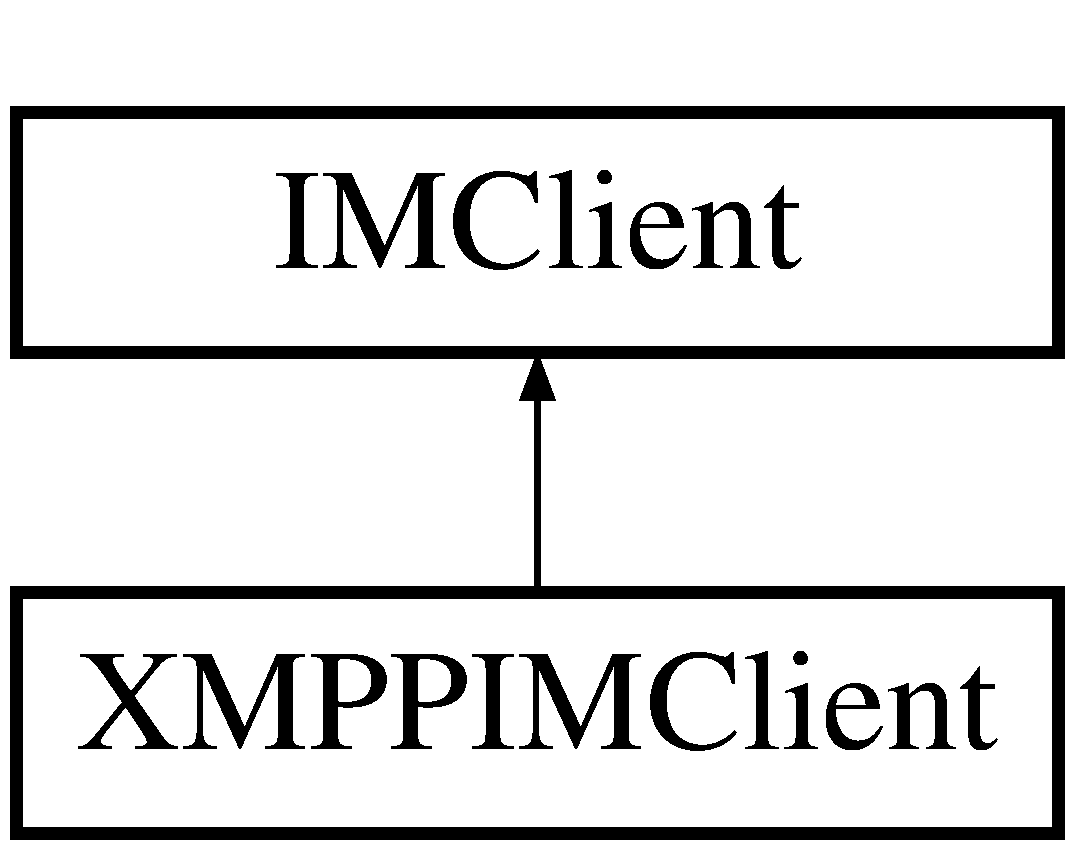
\includegraphics[height=2cm]{classXMPPIMClient}
\end{center}
\end{figure}
\subsection*{Signals}
\begin{DoxyCompactItemize}
\item 
\hypertarget{classXMPPIMClient_a374a5a7a31bfbb09cd6d3bd86c0b506e}{
void {\bfseries connected} ()}
\label{classXMPPIMClient_a374a5a7a31bfbb09cd6d3bd86c0b506e}

\item 
\hypertarget{classXMPPIMClient_a5499b021b2c9140775335583346ba53f}{
void {\bfseries disconnected} ()}
\label{classXMPPIMClient_a5499b021b2c9140775335583346ba53f}

\item 
\hypertarget{classXMPPIMClient_a566e19792d539ca5e45d0436ca8321c6}{
void {\bfseries gotMsg} (QString from, QString message)}
\label{classXMPPIMClient_a566e19792d539ca5e45d0436ca8321c6}

\item 
\hypertarget{classXMPPIMClient_af8f0aa177ce72d26718a67457ae2139b}{
void {\bfseries error} (QString errorMsg)}
\label{classXMPPIMClient_af8f0aa177ce72d26718a67457ae2139b}

\end{DoxyCompactItemize}
\subsection*{Public Member Functions}
\begin{DoxyCompactItemize}
\item 
\hypertarget{classXMPPIMClient_a8b42298615c65362800b338eaa01566d}{
{\bfseries XMPPIMClient} (\hyperlink{classIMAccount}{IMAccount} \&account)}
\label{classXMPPIMClient_a8b42298615c65362800b338eaa01566d}

\item 
\hypertarget{classXMPPIMClient_aa84fff629e311842be3461d3f9dcad18}{
void {\bfseries sendMsg} (QString target, QString message)}
\label{classXMPPIMClient_aa84fff629e311842be3461d3f9dcad18}

\item 
\hypertarget{classXMPPIMClient_a2dec1bfd485a5e1ee691ad4a11bf5b77}{
QStringList {\bfseries getPresence} ()}
\label{classXMPPIMClient_a2dec1bfd485a5e1ee691ad4a11bf5b77}

\item 
\hypertarget{classXMPPIMClient_a95bc16bff71222c54758c66c828db124}{
void {\bfseries login} ()}
\label{classXMPPIMClient_a95bc16bff71222c54758c66c828db124}

\item 
\hypertarget{classXMPPIMClient_af517015c407413a984bdec34a589ae23}{
void {\bfseries logout} ()}
\label{classXMPPIMClient_af517015c407413a984bdec34a589ae23}

\end{DoxyCompactItemize}


The documentation for this class was generated from the following files:\begin{DoxyCompactItemize}
\item 
adapter/adapter.h\item 
adapter/adapter.cpp\item 
adapter/examples/msg/moc\_\-adapter.cpp\end{DoxyCompactItemize}

\printindex
\end{document}
